\subsection{Directional diffusion}

The regular diffusion approach will present noticeable artifacts. These typically occur at high-contrast edges of the image. Because the diffusion kernel equally weighs pixels from all directions it creates a blur effect and is unable to properly propogate edges into the unknown regions. This effect can be seen in figure \ref{fig:artifacts}. To help resolve this problem we use directional kernels that weigh pixels from certain directions more heavily. To do this we divide the image into separate patches. For each patch we infer the general directionality by using a heuristic. We construct a directional kernel for the found directionality. Then we apply this kernel to do the inpainting for that specific patch.

We construct the directional kernel $K_\theta$ starting with a diagonal kernel $K_{\text{diag}}$. This kernel is converted to a $3\times 3$ image which is rotated by $\theta\degree$ and cropped to obtain a new $3\times 3$ image representing the rotated kernel. Bicubic interpolation is used to smooth the intermediate values.

Test

\begin{figure*}
	\centering
	\begin{subfigure}[b]{0.3\textwidth}
		\centering
		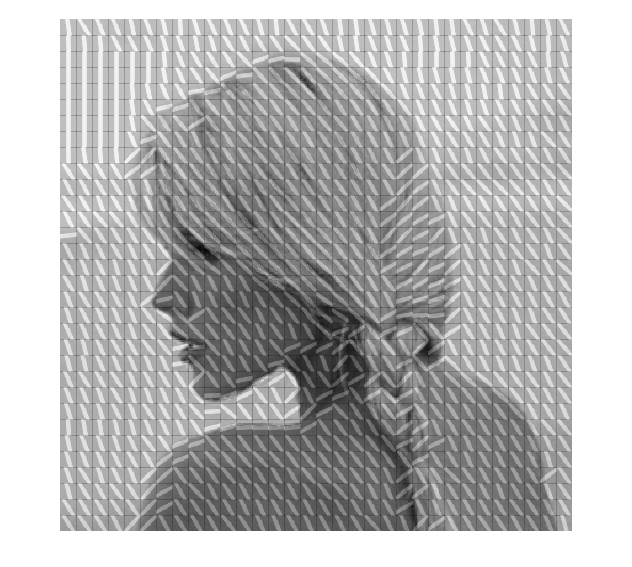
\includegraphics[clip, trim=2cm 0cm 2cm 0cm, width=0.9\textwidth]{figures/claudia-32x32}
		\caption{The claudia image.}
		\label{fig:claudia}
	\end{subfigure}
	\begin{subfigure}[b]{0.3\textwidth}
		\centering
		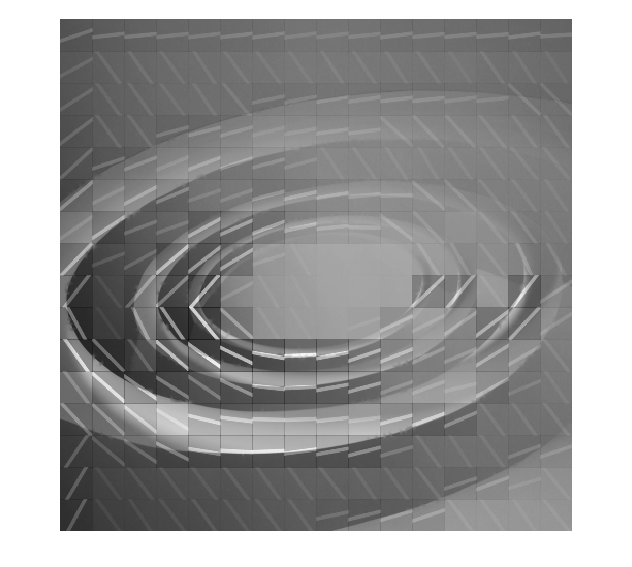
\includegraphics[clip, trim=2cm 0cm 2cm 0cm, width=0.9\textwidth]{figures/spiral-32x32}
		\caption{The spiral image.}
		\label{fig:spiral}
	\end{subfigure}
	\begin{subfigure}[b]{0.3\textwidth}
		\centering
		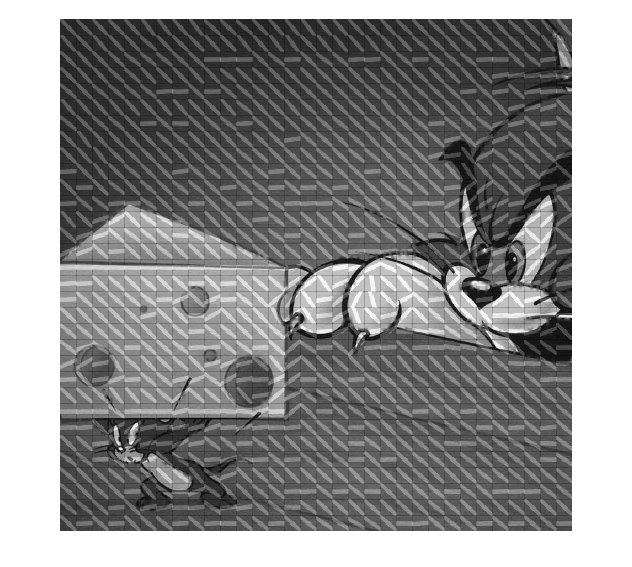
\includegraphics[clip, trim=2cm 0cm 2cm 0cm, width=0.9\textwidth]{figures/tomandjerry-32x32}
		\caption{The tom and jerry image.}
		\label{fig:spiral}
	\end{subfigure}
	
	\caption{The directionality of 32x32 pixel patches shown as white lines after the first diffusion stage.}
	\label{fig:directionality}
\end{figure*}